\documentclass[]{article}
\usepackage[letterpaper, margin=1in]{geometry}
\twocolumn
\usepackage{stfloats}
\usepackage{graphicx}
\usepackage{hyperref}
\hypersetup{
	colorlinks=true,
	linkcolor=blue,
	filecolor=magenta,      
	urlcolor=cyan,
}
%opening
\title{Gamma Radiation preparation report}
\author{Tal Silverwater}
\date{}

\begin{document}

\maketitle


\begin{table*}[!b]
	\centering
	\begin{tabular}{||c | c c c c c||} 
		\hline
		Nucleon & Mass & Spin & Magnetic Moment & Radius & Charge \\ [0.5ex] 
		\hline
		Proton & $1.00727647 u$ & $\frac{1}{2}\hbar$ & $2.7928474*\frac{e\hbar}{2m_p}$ & $10^{-15}m$ & $1e$ \\ 
		\hline
		Neutron & $1.00866490 u$ & $\frac{1}{2}\hbar$ & $-1.913043*\frac{e\hbar}{2m_p}$ & $10^{-15}m$ & 0  \\
		\hline
		
	\end{tabular}
	\caption{This table explains the property's of protons and neutrons}
\end{table*}

\section{General subjects in nuclear \\ physics}
\subsection{Typical sizes}

The typical radius of a nucleus is: $$R=1*10^{-15}m=1fermi=1fm$$
The typical radius of a atom is: $$R=1*10^{-10}m=1\AA$$
%can add more like forces and time scales

\subsection{Nuclear structure}

Rutherford has found in his experiments that the atom has a dense core in the middle (the nucleus), surrounded by a cloud of electrons.
The size of the nucleus for an aluminum atom is: $$r_{nucleus}=3*10^{-15}m$$ (found by Rutherford).
Since Rutherford experiments showed that the radius of the nucleus is: $$R=r_{0}A^{-\frac{1}{3}}$$ where A is the atomic mass number (number of protons times number of neutrons) and: $$r_0=1.2*10^{-15}m=1.2fm$$

\subsection{Components of the nuclues and \\ their property's}

The nucleus is made out of protons and neutrons. These particles are called hadrons and they are composed from Quarks. The protons are made of 2 up quarks and one down quark and the neutron is made out of two down quarks and one up quark.The property's of these particles are detailed in table 1.


\subsection{Forces in the nucleus}

There are two main forces inside the atomic nucleus:

1) The electromagnetic force, that acts between two charged particles according to: $$F_{12}=\frac{kq_1q_2}{|\vec{r}|^2}\hat{r}$$ This force is a repellent force in the nucleus because all the protons are positively charged, and therefore works in order to disassemble the nucleus.

2) The strong force, which is a force pulling all the parts of the nucleus together. This force is short distance which leads to a finite nucleus. It is much stronger then the coulomb force in short distances (for two protons with a distance of 2 fm the coulomb force is 60 N and the strong force is $2*10^{3} N$), but if the distance is really short the strong force is repulsive. This force is independent of charge, and dependent on spin. For equations and explanation see Ohanian Modern Physics page 351 (might be added later).

\subsection{The Liquid-Drop model}

This model is based on the similarity of intermolecular forces and the strong force, suggesting the nucleus acts like a liquid (can't be a solid because of zero point energy). In that view the nucleus is an almost incompressible fluid with constant density. This model leads to an approximated formula for the binding energy of the nuclei that depends on A and Z (atomic mass and number of protons). The binding energy term is: $$a_1A-a_2A^{2/3}$$ where $a_1$ and $a_2$ is a positive constant. The electrostatic potential can be written as: $$-a_3\frac{Z^2}{A^{1/3}}$$ where $a_3$ is an adjustable constant. The quantum mechanical correction gives: $$-a_4\frac{(A-2Z)^2}{A}$$ which is called the asymmetry energy. In total the binding energy B is: $$B=a_1A-a_2A^{2/3}-a_3\frac{Z^2}{A^{1/3}}-a_4\frac{(A-2Z)^2}{A}$$ From experiments we find: $$a_1=15.753Mev$$ $$a_2=17.804Mev$$ $$a_3=0.7103Mev$$ $$a_4=94.77Mev$$ This is called Weizs\"acker's semiempirical formula for binding energy. The formula for the mass is: $$M=Zm_H+(A-Z)m_n-\frac{B}{c^2}$$ where $m_H$ is equal to $Z(m_p+m_e)$ (you can plug in values and get eq 44 in page 357).
This approximation is good for large nuclei and is not expected to work for small A's. (Note- the larger B is the atom is more stable and when negitive the atom will burst apart). The nucleus is most stable when $\frac{\partial M}{\partial Z}=0$. Solving for Z we get: $$Z=\frac{A}{2+0.01499A^{2/3}}$$

\subsection{Basic idea of shell model}

The Liquid-Drop model isn't quantum and therefore misses important aspects of the nucleus,like the quantization of the angular momentum. Every nucleus has a spin which is a multiple of $\frac{1}{2}\hbar$. It also misses the energy levels of the nucleus, which is a potential sorce of $\gamma$ radiation.\\
The shell model attempts to calculate the the energy levels of the protons and neutrons in a nucleus under the assumption that the net force on every nucleon is approximated by an average central force. The idea is that nucleons can only be scattered near the nuclear surface (from the exclusion principal. more detailed in page 360). This means there is no force in the nucleus and very strong forces on the surface.

\section{Radioactivity}
\subsection{Statistics of radiation}

The statistics that describe radiation is given by the half-life formula: $$N(t)=N_0*(\frac{1}{2})^{t/\tau}$$ where $N(t)$ is the number of particles at time t, $N_0$ is the initial number of particles and $\tau$ is the half-life time.

\subsection{Background radiation}

This kind of radiation is ionizing, and is present in the environment. Background radiation originates from a variety of sources, both natural and artificial. Sources include cosmic radiation, and environmental radioactivity from such as naturally occurring radioactive materials including radon and radium, and fallout from nuclear weapons testing and nuclear accidents.

\section{$\alpha$ $\beta$ and $\gamma$ radiation}
\subsection{The type of radiation and its \\ emission process}
\subsubsection{$\alpha$ decay}

$\alpha$ particles are a nucleus of a helium 4 atom and is comprised of 2 protons and 2 neutrons. These particles are emitted when a massive and/or unstable particle break apart. 
There are 2 reasons why these particles are emitted (instead of protons, neutrons...):

1) Emission of $\alpha$ particles conserves the wave-function symmetry, which prevents a particle from spontaneously changing from exhibiting Bose–Einstein statistics (if it had an even number of nucleons) to Fermi–Dirac statistics (if it had an odd number of nucleons) or vice versa.

2) $\alpha$ particles have really high binding energy. This means it will not tend to break apart. the result is that heavy elements have enough energy in them to create this particle while other models of decay require additional energy. \\
The mechanism that explains $\alpha$ decay is quantum tunneling. In this process the $\alpha$ particle teleports out of the large nucleus to a point where the strong force is not strong enough to pull the $\alpha$ particle back, and then the electromagnetic force violently pushes the $\alpha$ particle away.
Mathematically, the coulomb potential energy of the alpha particle (charge $2e$) in the field of the daughter nucleus (charge $Ze$) when $r>R$ is: $$U(r)=\frac{2Ze^2}{4\pi \epsilon_0r}$$ when $r<R$: $$U(r)=-U_0$$ ($U_0$ not critical). When adding that the probability to tunnel is: $$P=e^{-\frac{4\pi}{\hbar}\frac{Ze^2}{4\pi \epsilon_0}\frac{1}{\nu_\alpha}}$$ where $\nu_\alpha$ is the speed of the ejected alpha particle. From that we get that the mean life (half-life formula with e insted of 1/2) is: $$\tau=\frac{2R}{\nu_{in}}e^{\frac{4\pi}{\hbar}\frac{Ze^2}{4\pi \epsilon_0}\frac{1}{\nu_\alpha}}$$ where $\nu_{in}$ is the velocity of the $\alpha$ particle in the nucleus.

\subsubsection{$\beta$ decay}

$\beta$ particles are high energy electrons ($\beta^-$) or positrons ($\beta^+$). 
The emission process for a $\beta^-$ happens when an unstable atomic nucleus with an excess of neutrons converts a neutron into a proton while emitting an electron and a electron anti-neutrino $n\rightarrow p+e^-+\bar{\nu}_e$. This process is mediated by the weak interaction. The neutron turns into a proton through the emission of a virtual $W^-$ boson. At the quark level, $W^-$ emission turns a down quark into an up quark, turning a neutron into a proton. The virtual $W^-$ boson then decays into an electron and an antineutrino. This process happens in fission byproducats.\\
The emission process for a $\beta^+$ is explained by\\
$p\rightarrow n+e^++\nu_e$. This decay can only happen inside nuclei when the absolute value of the binding energy of the daughter nucleus is greater than that of the parent nucleus, i.e., the daughter nucleus is a lower-energy state.

\subsubsection{$\gamma$ decay}

$\gamma$ radiation is an electromagnetic wave with a frequency of more then $10^{19}Hz$.
One source for $\gamma$ rays is $\gamma$ decay. When a heavy and/or unstable atom goes through $\alpha$ or $\beta$ decay, the resulting nucleus usually is in a high energy state. The nucleus then decays to a lower energy state while emitting a $\gamma$ ray photon. The emission takes $10^{-12}sec$.
There are other sources of gamma radiation. For example: Cosmic rays, Cosmic rays, Gamma-ray bursts...

\subsection{How does the spectrum look like}

The spectrum for $\beta$ particles is broad because the neutrino can have different amounts of energy. A illustration can be seen in figure 1 \\ For alpha particles the spectrum (for one atom) are sharp lines (usually 1 of 2). These lines indicates the energy levels of the atoms that relese them. You can see Figure 2 for an illustration.
\begin{figure}
	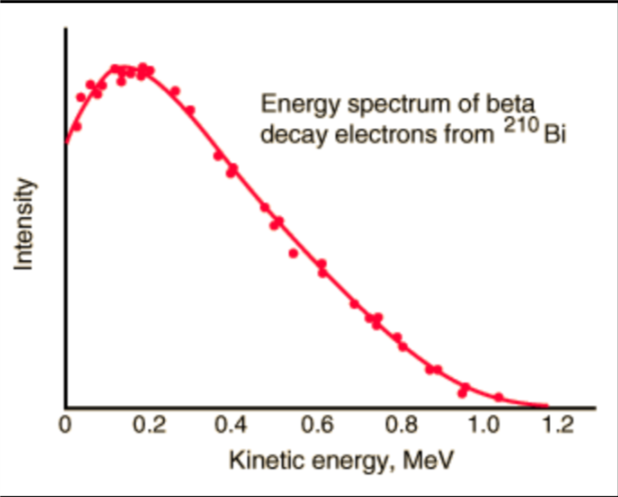
\includegraphics[width=\linewidth]{beta-decay-spectrum.png}
	\caption{The shape of this energy curve depends on what fraction of the reaction energy that is carried by the electron or neutrino.}
	\label{fig:beta spectrum}
\end{figure}
\begin{figure}
	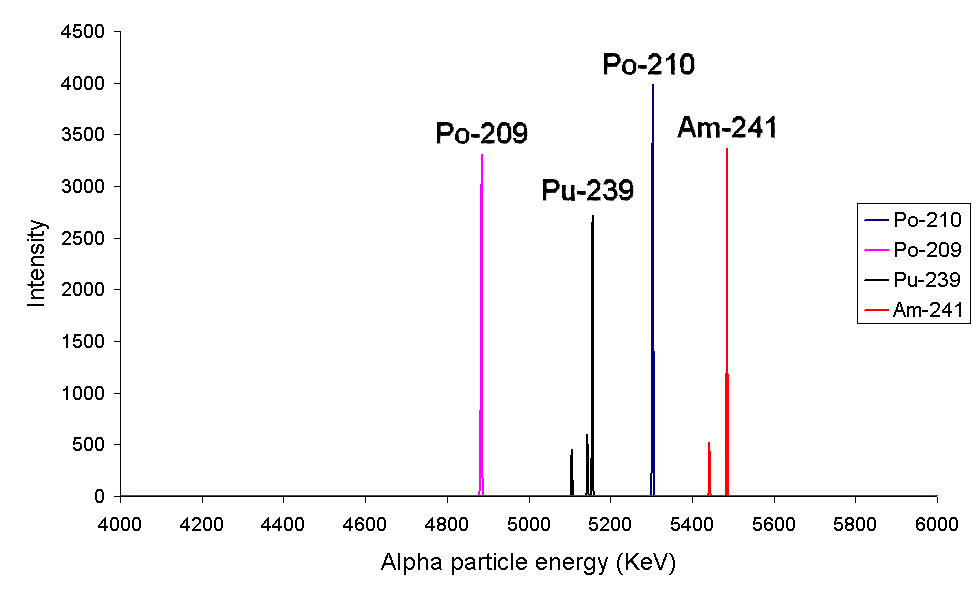
\includegraphics[width=\linewidth]{Alpha1spec.png}
	\caption{Intensity against alpha energy for four isotopes, note that the line width is narrow and the fine details can be seen}
	\label{fig:Alpha spectrum}
\end{figure}
For gamma radiation we expect to get "delta-functions", but because of different effects concerning interactions with matter we will probably see noise (more on these effects later).

\subsection{Interaction with matter}
\subsubsection{$\alpha$ particles}

There are different interaction of $\alpha$ particles with matter. One example is when a $\alpha$ particle hits a heavy nucleus and merges with it. This may result in a unstable atom which may break apart (a fission reaction).
Another option is that the $\alpha$ particle collides with a different atom (can be air or surrounding metirial). With this model we can define the stoping power of a metrical.  The linear stopping power of material is defined as the ratio of the differential energy loss for the particle within the material to the corresponding differential path length: $$S(T)=-\frac{dT}{dx}=n_{ion}\bar{I}$$ where T is the kinetic energy of the charged particle, $n_{ion}$ is the number of electron-ion pairs formed per unit path length, and I denotes the average energy needed to ionize an atom in the medium. For charged particles, S increases as the particle velocity decreases. The classical expression that describes the specific energy loss is known as the Bethe formula (there in a non-relativistic formula, but here we have the relativistic one): $$S(T)=\frac{4\pi Q^2e^2nZ}{m\beta^2c^2}\left[ln\left(\frac{2mc^2\gamma^2\beta^2}{\bar{I}}\right)x-\beta^2\right]$$ In this expression, m is the rest mass of the electron, $\beta$ equals to v/c, what expresses the particle’s velocity relative to the speed of light, $\gamma$ is the Lorentz factor of the particle, Q equals to its charge, Z is the atomic number of the medium and n is the atoms density in the volume. 

\subsubsection{$\beta$ particles}

A $\beta$ particle can do a elastic interaction with a nucleus which can change the direction of the $\beta$ particle. This results in the particle zig-zaging around. They can also lose their energy from emitting electomagnetic radiation (a process known as Bremsstrahlung). Another method is when they move faster then the speed of light in the medium they're in. This causes electromagnetic radiation called Cherenkov radiation. $\beta^+$ particles can also annihilate with an electron.(There is an equation like Bethe formula for $\beta$ particles but is is very complicated. also there are equations for Bremsstrahlung and Cherenkov radiation, see \href{http://www.nuclear-power.net/nuclear-power/reactor-physics/interaction-radiation-matter/interaction-beta-radiation/}{Here})

\section{$\gamma$ radiation interaction with matter}

There are three kinds of interaction with matter:

1) Photoelectric effect: when a high energy photon hits a material it can eject an electron from that material. That happens usually in the lower part of the $\gamma$ spectrum. The main equation that describes this interaction is: $$E_e=h\nu-E_b$$ where $E_e$ is the kinetic energy of the electron, h is Plank's constant, $\nu$ is the frequency of the of the light ($\gamma$ ray photon) and $E_b$ is the binding energy of the electron to the material (This equation is just an equation of conservation of energy).

2) Compton scattering: this happens in intermediate energy's, when a $\gamma$ ray hits a atomic electron. This causes the $\gamma$ ray to scatter in a way such that the frequency depends on the scattering angle. The main equation is derived from the fact that for a photon $E=p_{photon}c=\frac{h}{\lambda}$. From conservation of momentum and energy we can get: $$\Delta \lambda =\lambda '-\lambda=\frac{h}{m_ec}(1-\cos(\theta))$$ where $\lambda$ is the initial wavelength of the photon, $\lambda'$ is the wavelength of the photon after scattering, h is Plank's constant, $m_e$ is the electron rest mass, c is the speed og light and $\theta$ is the scattering angle for the photon.

3) At high energy the $\gamma$ ray photon can be converted to matter by creating an particle anti-particle pair (like an electron positron). For that to happen the energy of the photon needs to be above a threshold energy (for an electron positron pair that energy is $1.02Mev$). (This interaction also needs to conserve energy and momentum)

\section{How does the detector work}













\end{document}
